\documentclass[aspectratio=169]{beamer}
\usetheme{metropolis}
\usepackage{bm}
\usepackage{xcolor}
\colorlet{shadecolor}{blue!15}
\usepackage{framed}
\usepackage{amsthm}
\usepackage[utf8]{inputenc}
\usepackage[spanish, es-noshorthands]{babel}
\usepackage{subfig}
\usepackage{graphicx}
\usepackage{minted}


% Macros
\newcommand{\bx}{\bm{x}}
\newcommand{\bX}{\bm{X}}
\newcommand{\bw}{\bm{w}}
\newcommand{\bW}{\bm{W}}
\newcommand{\bz}{\bm{z}}
\newcommand{\bZ}{\bm{Z}}
\newcommand{\bv}{\bm{v}}
\newcommand{\bV}{\bm{V}}
\newcommand{\bH}{\bm{H}}
\newcommand{\bh}{\bm{h}}
\newcommand{\bSigma}{\bm{\Sigma}}
\newcommand{\bpi}{\bm{\pi}}
\newcommand{\bLambda}{\bm{\Lambda}}
\newcommand{\bmu}{\bm{\mu}}
\newcommand{\btheta}{\bm{\theta}}
\newcommand{\bnu}{\bm{\nu}}
\DeclareMathOperator*{\argmax}{arg\,max}
\DeclareMathOperator*{\argmin}{arg\,min}
\newcommand\E[2]{\mathbb{E}_{#1}\Big[#2\Big]}
\newcommand\KL[2]{KL\Big(#1 \bigm| #2\Big)}
\newcommand{\bigCI}{\mathrel{\text{\scalebox{1.07}{$\perp\mkern-10mu\perp$}}}}
\newcommand{\bigCD}{\centernot{\bigCI}}
\usepackage{pgfplots}

% TikZ
\usepackage{tikz}
\usetikzlibrary{positioning}
\usetikzlibrary{bayesnet}
\usetikzlibrary{shapes.geometric}
\usetikzlibrary{decorations.text}
\usetikzlibrary{calc,intersections}
\usetikzlibrary{arrows.meta,
                quotes,
                shapes.geometric}

\newcommand\Fontvi{\fontsize{8}{7.2}\selectfont}

\title{Modelos estadísticos con métodos variacionales}
\subtitle{Doble Grado en Ingeniería Informática y Matemáticas}
\date{\today}
\author{Luis Antonio Ortega Andrés}
\institute{Trabajo Fin de Grado \\\\\\ \emph{E.T.S. de Ingenierías Informática y de Telecomunicación} \\ \emph{Facultad de Ciencias}}

\usepackage[absolute,overlay]{textpos}
\titlegraphic{
  \begin{textblock*}{5cm}(9.5cm,4.8cm)
    
\includegraphics[width=5cm]{ugr}
  \end{textblock*}
}


\begin{document}
  \maketitle

  \begin{frame}{Índice}
    \begin{columns}
      \begin{column}{0.5\textwidth}
         % Inferencia estadística\\
         % \quad Enfoques\\
         Inferencia variacional\\
         \quad Algoritmo EM\\
         \quad Algoritmo CAVI\\
         \quad Familia exponencial\\
         \vspace*{0.2cm}
         Redes Bayesianas\\
         % \quad D-separación y D-conexión\\
         \quad Algoritmo EM\\
         \quad Algoritmo paso de mensajes\\
       \end{column}
       \begin{column}{0.5\textwidth}
         Modelos\\
         \quad Mixtura de Gaussianas\\
         \quad Asignación latente de Dirichlet \\
         \quad Reducción de dimensionalidad\\
         \vspace*{0.2cm}
         Casos prácticos\\
         \quad InferPy\\
         \quad BayesPy\\
         \quad Scikit-Learn\\
       \end{column}
     \end{columns}
  \end{frame}

  \begin{frame}{Introducción}
    Los métodos variacionales permiten la resolución de problemas de inferencia con variables ocultas, tanto con enfoque Bayesiano como basado en verosimilitud. Han aumentado notablemente los modelos estadísticos en los que se puede hacer inferencia.

    Las variables ocultas pueden ser parámetros bajo un modelo Bayesiano.

    La utilización de estructuras de red Bayesiana y la familia exponencial simplifican notablemente la tarea de inferencia.

    Modelos concretos como la mixtura de Gaussianas, localización latente de Dirichlet y análisis de componentes principales pueden ser estudiados mediante la utilización de lenguajes de programación especializados.
  \end{frame}

    \begin{frame}{Divergencia Kullback-Leibler}
    Sean \(P\) y \(Q\) dos distribuciones de probabilidad sobre el mismo espacio probabilístico, su \emph{divergencia de Kullback-Leibler} \(\KL{Q}{P}\) mide la ``diferencia'' de \(Q\) a \(P\)
    \[
      \KL{Q}{P} = \E{Q}{\log Q(x) - \log P(x)}.
    \]
    \begin{shaded}
      La divergencia de Kullback-Leibler es siempre no negativa.
    \end{shaded}
  \end{frame}

  \begin{frame}{El problema}
    \begin{itemize}
      \item Un conjunto de variables observadas i.i.d \(\bX = (X_{1},\dots,X_{N})\).
      \item Variables ocultas globales \(\btheta\) y variables ocultas locales \(\bZ = (Z_{1},\dots,Z_{N})\).
      \item La distribución conjunta factoriza como
        \[
        P(\bx, \bz, \btheta) = P(\btheta)\prod_{n=1}^{N}P(x_{n}, z_{n} \mid \btheta).
        \]
    \end{itemize}
    \begin{shaded}
      Las variables ocultas pueden ser tratadas como variables o como parámetros.
    \end{shaded}
    \textbf{Objetivo:} calcular
    \[
      P(\btheta, \bz \mid \bx) = \frac{P(\btheta, \bz, \bx)}{\int_{\btheta, \bz}P(\btheta, \bz, \bx)}.
    \]
  \end{frame}


  \section{Inferencia variacional}
  \begin{frame}{Inferencia variacional}

    Resuelve el problema de inferencia mediante uno de \emph{optimización}:
    \begin{shaded}
      Dada una familia de distribuciones \(\mathcal{Q}\) sobre el conjunto de variables ocultas \(\bZ\), encontrar
      \[
        Q^{opt} = \argmin_{Q \in \mathcal{Q}} \KL{Q(\bz)}{P(\bz \mid \bx)}.
      \]
    \end{shaded}

    El problema se afronta mediante técnicas de aprendizaje automático como \emph{gradiente descendente} o \emph{descenso coordinado}.
  \end{frame}

  \begin{frame}{Cota inferior para la evidencia}
    Utilizando la positividad de la divergencia de Kullback-Leibler, se obtiene una cota inferior para la evidencia:
    \[
      \KL{Q(\bz)}{P(\bz \mid \bx)} \geq 0
    \]
    \[
      \Updownarrow
    \]
    \[
      \log P(\bx) \geq \underbrace{- \E{Q(\bz)}{\log Q(\bz)}}_{\text{Entropía}} + \underbrace{\E{Q(\bz)}{\log P(\bx, \bz)}}_{\text{Energía}} = ELBO(Q).
    \]
  \end{frame}


  \begin{frame}{ Algoritmo Esperanza-Maximización}
    No considera distribución sobre los parámetros.
    \[
      ELBO(Q, \btheta) = \underbrace{- \E{Q(\bz)}{\log Q(\bz)}}_{\text{Entropía}} + \underbrace{\E{Q(\bz)}{\log P(\bx, \bz \mid \btheta)}}_{\text{Energía}}.
    \]
    Dos pasos iterativos:
    \begin{itemize}
      \item \textbf{Paso E}: Fijado el parámetro \(\btheta\),
        \[
        Q^{new}(\bz) = \argmax_{Q} ELBO(Q, \btheta) = P(\bz \mid \bx, \btheta).
        \]
      \item \textbf{Paso M}: Fijada la distribución \(Q\),
        \[
        \btheta^{new} = \argmax_{\btheta} ELBO(Q, \btheta) = \argmax_{\btheta} \E{Q(\bz)}{\log P(\bx, \bz \mid \btheta)}.
        \]
    \end{itemize}
  \end{frame}

  \begin{frame}
    \begin{shaded}
      El algoritmo EM incrementa la verosimilitud.
    \end{shaded}
    \[
      \log P(\bx \mid \btheta ) \geq - \E{Q(\bz)}{\log Q(\bz)} + \E{Q(\bz)}{\log P(\bx, \bz \mid \btheta)}.
    \]
    \[
      \Downarrow \ \text{Paso E}
    \]
    \[
      \log P(\bx \mid \btheta ) = - \E{P(\bz \mid \bx, \btheta)}{\log P(\bz \mid \bx, \btheta)} + \E{P(\bz \mid \bx, \btheta)}{\log P(\bx, \bz \mid \btheta)}.
    \]
    \[
      \Downarrow \ \text{Paso M}
    \]
    \[
      \log P(\bx \mid \btheta^{new} ) \geq - \E{P(\bz \mid \bx, \btheta)}{\log P(\bz \mid \bx, \btheta)} + \E{P(\bz \mid \bx, \btheta)}{\log P(\bx, \bz \mid \btheta^{new})}.
    \]
    \begin{shaded}
      Converge a un máximo local.
    \end{shaded}
  \end{frame}

  \begin{frame}{Algoritmo de ascenso coordinado en inferencia variacional}
    La familia de distribuciones de \emph{campo medio} factoriza como producto de marginales:
    \[
      Q(\bz) = \prod_{m=1}^{M}Q(z_{m}).
    \]
    \begin{columns}
      \begin{column}{0.5\textwidth}
        \begin{itemize}
          \item Pueden capturar cualquier distribución marginal.
          \item No pueden capturar correlación entre variables.
        \end{itemize}
      \end{column}
      \begin{column}{0.5\textwidth}
        \begin{tikzpicture}
          \pgfplotsset{ticks=none}
          \begin{axis}[
            axis lines = middle,
            xmin=-10, xmax=10, ymin=-10, ymax=10,
            axis equal,
            xlabel = $z_{1}$,
            ylabel = {$z_{2}$},
            yticklabels={,,},
            ]
            \draw[rotate around={45:(0,0)}, color=blue!50, fill=blue!20, very thick, opacity=0.7] (140,0) ellipse (7 and 2);
            \filldraw[color=purple!50, fill=purple!20, very thick, opacity=0.7]  (100,100) circle (3);
          \end{axis}
        \end{tikzpicture}
      \end{column}
    \end{columns}
  \end{frame}

  \begin{frame}
    El algoritmo de ascenso coordinado se basa en:
    \begin{itemize}
      \item Los parámetros se consideran variables ocultas \(\btheta \subset \bZ\).
      \item La familia de distribuciones \(\mathcal{Q}\) del problema de optimización es la familia de campo medio.
      \item La distribución marginal de cada variable se actualiza cada vez.
    \end{itemize}
    \[
      Q^{new}(z_{m}) = \argmax_{Q \in \mathcal{Q}} ELBO(Q)
    \]
    \[
      \Downarrow
    \]
    \[
      Q^{new}(z_{m}) \propto \exp \E{Q_{\backslash m}}{\log P(z_{m} \mid \bz_{\backslash m}, \bx)} \propto \exp \E{Q_{\backslash m}}{\log P(\bz, \bx)}
    \]
  \end{frame}

  \begin{frame}{Familia exponencial}
    \begin{shaded}
      Una variable aleatoria \(X\) sigue una distribución en la \emph{familia exponencial} con parámetros \(\btheta\) si y solo si existen \(\bm{T}, \bm{\eta}\) y \(\psi\) tales que
      \[
        P(x \mid \btheta) = h(x) \exp \Big( \bm{\eta}(\btheta)^{T}\bm{T}(x) - \psi(\btheta)\Big).
      \]
    \end{shaded}
    \begin{itemize}
      \item \(\bm{T}\) es el estadístico natural de \(X\). \emph{Teorema de Fisher-Neyman}.
      \item \(\bm{\eta}\) se denomina la función paramétrica de la distribución.
      \item \(\psi\) asegura normalización logarítmica
        \[
        \psi(\btheta) = \log \int_{x} h(x)\exp \Big( \bm{\eta}(\btheta)^{T}\bm{T}(x) \Big).
        \]
    \end{itemize}
  \end{frame}

  \begin{frame}{Distribuciones conjugadas}
    Si la distribución a \emph{posteriori} y la distribución a \emph{priori} pertenecen a la misma familia, se denominan \emph{conjugadas} y la distribución a priori se dice \emph{distribución a priori conjugada} de la verosimilitud.
    \[
      \underbrace{P(\btheta \mid \bx)}_{posteriori} = \frac{\overbrace{P(\bx \mid \btheta)}^{verosimilitud}\overbrace{P(\btheta)}^{priori}}{P(\bx)}.
    \]
  \end{frame}

  \begin{frame}{Modelos condicionalmente conjugados}

    Se consideran distribuciones conjugadas en la familia exponencial.

    Las actualizaciones de las distribuciones variacionales \(Q^{new}(z_{n})\) y \(Q^{new}(\btheta)\) consisten en actualizar la \emph{función paramétrica de la distribución} \(\bm{\eta}\).

    Estas actualizaciones puede calcularse de forma eficiente, calculando esperanzas de los estadísticos suficientes.

  \end{frame}

  \section{Redes Bayesianas}

  \begin{frame}{Red Bayesiana}
    \begin{shaded}
      Una \emph{red de creencia o red Bayesiana} es una pareja \((G,P)\) formada por un grafo dirigido acíclico \(G\) y una distribución de probabilidad \(P\) tal que existe una correspondencia entre variables y nodos verificando:
      \[
        P(x_{1},\dots,x_{N}) = \prod_{n=1}^{N}P(x_{n}\mid pa(x_{n})).
      \]
    \end{shaded}
    \begin{columns}
      \begin{column}{0.5\textwidth}
        \centering
        \begin{tikzpicture}[
          node distance=1cm and 1cm,
          mynode/.style={draw,circle,text width=0.4cm,align=center}
          ]

          \node[mynode] (1) {\(X_1\)};
          \node[mynode,right=of 1] (2) {\(X_2\)};
          \node[mynode,right=of 2] (3) {\(X_3\)};

          \path (3) edge[-latex][bend right] (1)
          (3) edge[-latex] (2)
          ;
        \end{tikzpicture}
        \[
          P(x_{1}, x_{2}, x_{3}) = P(x_{1} \mid x_{3})P(x_{2}\mid x_{3})P(x_{3}).
        \]
      \end{column}
      \begin{column}{0.5\textwidth}
        La inferencia se puede realizar de forma eficiente mediante los conocidos algoritmos de propagación en problemas con un gran número de variables.
      \end{column}
    \end{columns}
  \end{frame}

  \begin{frame}{Algoritmo de paso de mensajes}
    Proceso de paso de mensajes entre los nodos de la red.
    \begin{itemize}
      \item Familia variacional de campo medio.
        \[Q(\bz) = \prod_{m=1}^{M}Q(z_{m}).\]
      \item Modelo condicionalmente conjugado en la familia exponencial.
      \item Ascenso coordinado en redes Bayesianas.
    \end{itemize}
  \end{frame}

  \begin{frame}
    La actualización de la distribución dada la red es:
    \[
      \log Q^{new}(z) = \E{Q_{\backslash Z}}{ \sum_{n=1}^N \log P(x_n \mid pa(x_n))} + \text{const.}
    \]
     La aportación de \(Z\):
    \[
        \log Q^{new}(z) = \E{Q_{\backslash Z}}{\log P(z \mid pa(z))} + \sum_{X \in ch(Z)} \E{Q_{\backslash Z}}{\log P(x \mid z,cp(z, x))} + \text{const.}
    \]
  \end{frame}

  \begin{frame}
      El mensaje de un nodo padre \( X \) a uno hijo \( Z \):
      \[
        \bm{m}_{X \to Z} = \E{Q}{\bm{T}_{X}(x)}.
      \]
      El mensaje de un nodo hijo \(X\) a un nodo padre \(Z\):
    \[
    \bm{m}_{X \to Z} = \bar{\bm{\eta}}_{X,Z}\Big(\E{Q}{\bm{T}_X(x)}, \{\bm{m}_{Y \to X}\}_{Y \in cp_{Z,X}}\Big),
    \]

    \centering
    \begin{tikzpicture}[
      node distance=0.5cm and 0.25cm,
      mynode/.style={draw,circle,text width=0.35cm,align=left}
      ]

      \node[mynode] (31) {\(X_{3}\) };
      \node[mynode, above left=of 31] (11) {\(X_{1}\) };
      \node[mynode, above right=of 31] (21) {\(X_{2}\) };
      \node[mynode, below right=of 21] (41) {\(X_{4}\) };
      \node[mynode, below left=of 31] (51) {\(X_{5}\) };
      \node[mynode, below right=of 31] (61) {\(X_{6}\) };

      \node[mynode, right =1.5cm of 41] (32) {\(X_{3}\) };
      \node[mynode, above left=of 32] (12) {\(X_{1}\) };
      \node[mynode, above right=of 32] (22) {\(X_{2}\) };
      \node[mynode, below right=of 22] (42) {\(X_{4}\) };
      \node[mynode, below left=of 32] (52) {\(X_{5}\) };
      \node[mynode, below right=of 32] (62) {\(X_{6}\) };

      \node[mynode, right =1.5cm of 42] (33) {\(X_{3}\) };
      \node[mynode, above left=of 33] (13) {\(X_{1}\) };
      \node[mynode, above right=of 33] (23) {\(X_{2}\) };
      \node[mynode, below right=of 23] (43) {\(X_{4}\) };
      \node[mynode, below left=of 33] (53) {\(X_{5}\) };
      \node[mynode, below right=of 33] (63) {\(X_{6}\) };


      \path (11) edge[-latex] (31)
      (21) edge[-latex] (31)
      (31) edge[-latex] (51)
      (31) edge[-latex] (61)
      (41) edge[-latex] (61)
      ;
      \path [bend left] (11) edge[-latex, orange] (31);
      \path [bend left] (21) edge[-latex, orange] (31);

      \path (12) edge[-latex] (32)
      (22) edge[-latex] (32)
      (32) edge[-latex] (52)
      (32) edge[-latex] (62)
      (42) edge[-latex] (62)
      ;
      \path [bend left] (42) edge[-latex, orange] (62);

      \path (13) edge[-latex] (33)
      (23) edge[-latex] (33)
      (33) edge[-latex] (53)
      (33) edge[-latex] (63)
      (43) edge[-latex] (63)
      ;
      \path [bend right] (63) edge[-latex, orange] (33);
      \path [bend right] (53) edge[-latex, orange] (33);

    \end{tikzpicture}
  \end{frame}

  \section{Modelos}
  \pgfmathdeclarefunction{gauss}{2}{%
    \pgfmathparse{1/(#2*sqrt(2*pi))*exp(-((x-#1)^2)/(2*#2^2))}%
  }
  \begin{frame}{Mixtura de Gaussianas}
    \begin{columns}
      \begin{column}{0.5\textwidth}
        La probabilidad de un punto se define como la suma de las probabilidades de pertenecer a cada Gaussiana por la probabilidad de dicho punto en ella.
      \end{column}
      \begin{column}{0.6\textwidth}
    \begin{tikzpicture}
      \begin{axis}[every axis plot post/.append style={
          mark=none,domain=-2:5,samples=50,smooth},
        axis x line*=bottom,
        axis y line*=left,
        enlargelimits=upper]
        \addplot {gauss(0,0.5)};
        \addplot {gauss(2,0.75)};
        \addplot {gauss(3, 0.4)};
      \end{axis}
    \end{tikzpicture}
    \end{column}
  \end{columns}
  \end{frame}

  \begin{frame}
    \begin{columns}
      \begin{column}{0.55\textwidth}
    \centering
    \begin{tikzpicture}[
      node distance=0.5cm and 1cm,
      mynode/.style={draw,circle,text width=0.5cm,align=center},
      hidden/.style={draw,circle,text width=0.8cm,align=center},
      param/.style={draw,text width=0.5cm,align=center, fill={rgb:black,1;white,6;blue,0.5}}
      ]

      \node[mynode] (mu) {\(\bm{\mu}\)};
      \node[mynode, right=of mu] (sigma) {\(\bm{\Lambda}\) };


      \node[mynode, below =of sigma] (z) {\(Z_{n}\)};
      \node[mynode, left =of z] (phi) {\(\bm{\pi}\)};
      \node[mynode,fill={rgb:black,1;white,2}, right =of z] (x) {\(X_{n}\)};

      \node[param,  above=of mu] (lambda) {\(m_{0}\)};
      \node[param, left=of lambda] (mu0) {\(\beta_{0}\)};
      \node[param, above=of sigma] (v) {\(\nu_{0}\)};
      \node[param, right=of v] (sigma0) {\(W_{0}\)};
      \node[param, left=of phi] (beta) {\(\alpha_{0}\)};

      \plate[inner sep=.3cm,xshift=.02cm,yshift=.2cm] {} {(z)(x)} {\(n=1,\dots,N\)}; %

      \path (mu) edge[-latex] (x)
      (sigma) edge[-latex] (x)
      (sigma) edge[-latex] (mu)
      (z) edge[-latex] (x)
      (beta) edge[-latex] (phi)
      (phi) edge[-latex] (z)
      (mu0) edge[-latex] (mu)
      (lambda) edge[-latex] (mu)
      (v) edge[-latex] (sigma)
      (sigma0) edge[-latex] (sigma)
      ;
    \end{tikzpicture}
  \end{column}
  \begin{column}{0.7\textwidth}
    \begin{itemize}
      \item \textbf{Pesos}: \(\bpi \sim \text{Dirichlet}(\alpha_{0})\).
      \item \textbf{Medias y precisiones: }\((\bmu, \bLambda) \sim \text{Gaussian-Wishart}(\beta_{0}, m_{0}, \nu_{0}, W_{0})\).
      \item \textbf{Componentes}: \(Z_{n} \mid \bpi \sim Categorica(\bpi)\).
      \item \textbf{Observaciones}:

        \(X_{n} \mid z_{n}, \bmu, \bLambda \sim \mathcal{N}(\mu_{z_{n}}, \Lambda_{z_{n}})\).
    \end{itemize}
  \end{column}
  \end{columns}
  \end{frame}

  \begin{frame}{Asignación latente de Dirichlet}
  \centering
  \begin{tikzpicture}[
    node distance=1.5cm and 1.5cm,
    mynode/.style={draw,circle,text width=0.7cm,align=center},
    param/.style={draw,text width=0.5cm,align=center,fill={rgb:black,1;white,6;blue,0.5} }
    ]

    \node[mynode,fill={rgb:black,1;white,2} ] (w) {\(W_{d,n}\)};
    \node[mynode, left=of w] (z) {\(Z_{d,n}\) };

    \node[mynode, left=of z] (theta) {\(\theta_{d}\)};
    \node[mynode, right=of w] (beta) {\(\beta_{k}\)};


    \node[param, left=of theta] (alpha) {\(\alpha\)};
    \node[param, right=of beta] (eta) {\(\eta\)};


    \plate[inner sep=.3cm,xshift=.02cm,yshift=.2cm] {plate1} {(z)(w)} {\(n = 1\dots N_{d}\)}; %

    \plate [inner sep=.15cm,xshift=-.01cm,yshift=.11cm]{} {(plate1)(theta)} {\(d = 1\dots D\)}; %

    \plate [inner sep=.3cm,xshift=.02cm,yshift=.2cm]{} {(beta)}{\(k=1,\dots,K\) };

    \path (z) edge[-latex] (w)
    (theta) edge[-latex] (z)
    (alpha) edge[-latex] (theta)

    (beta) edge[-latex] (w)
    (eta) edge[-latex] (beta)
    ;
  \end{tikzpicture}
  \begin{itemize}
    \item \textbf{Palabras por tema: }\(\beta_{k} \sim \text{Dirichlet}(\eta)\).
    \item \textbf{Temas por documento: }\(\theta_{d} \sim \text{Dirichlet}(\alpha)\).
    \item \textbf{Temas por documento y palabra: }\(Z_{d,n} \mid \theta_{d} \sim \text{Categorica}(\theta_d)\).
    \item \textbf{Palabras: }\(W_{d,n } \mid z_{d,n}, \bm{\beta} \sim \text{Categorica}(\beta_{z_{d,n}})\).
  \end{itemize}
  \end{frame}
  \begin{frame}{Reducción de dimensionalidad}
    \begin{shaded}
      Reducción de espacio \(D\) dimensional a uno \(K\) dimensional.
    \end{shaded}
    \begin{columns}
      \begin{column}{0.3\textwidth}
        \begin{tikzpicture}[
          node distance=1cm and 0.5cm,
          mynode/.style={draw,circle,text width=0.5cm,align=center},
          param/.style={draw,text width=0.5cm,align=center,  fill={rgb:black,1;white,6;blue,0.5}}
          ]

          \node[mynode] (theta) {\(\bm{W}\)};
          \node[mynode, below left=of theta] (zn) {\(Z_{n}\)};
          \node[mynode,  fill={rgb:black,1;white,2}, below right=of theta] (xn) {\(X_{n}\)};
          \node[param, right=of xn] (sigma) {\(\sigma\)};

          \plate[inner sep=.3cm,xshift=.02cm,yshift=.2cm] {} {(zn)(xn)} {\(n = 1\dots N\)}; %
          \path (theta) edge[-latex] (xn)
          (sigma) edge[-latex] (xn)
          (zn) edge[-latex] (xn)
          ;

        \end{tikzpicture}
      \end{column}
      \begin{column}{0.7\textwidth}
        \begin{itemize}
          \item \textbf{Transformación lineal: } \(\bm{W} \sim \mathcal{N}_{D \times K}(0, I)\).
          \item \textbf{Representación oculta: } \(Z_{n} \sim \mathcal{N}_{K}(0, I)\).
          \item \textbf{Representación observada: } \(X_{n} \mid \bm{W}, z_{n} \sim \mathcal{N}_{d}(\bm{W}z_{n}, \sigma I)\).
        \end{itemize}
      \end{column}
    \end{columns}
    \vspace*{0.5cm}
    \textbf{Modelo no lineal:} Red neuronal totalmente conectada de 2 capas.
    \[
      X_{n} \mid z_{n} \sim \mathcal{N}_{D}(f(z_{n}), \sigma I).
    \]
  \end{frame}

  \begin{frame}{Codificadores variacionales automáticos}
    \begin{columns}
      \begin{column}{0.5\textwidth}
        \textbf{Modelo paramétrico}

        Representación oculta
        \[
          Z_{n} \sim \mathcal{N}_{K}(0, I).
        \]
        Representación observada
        \[
          X_{n} \mid z_{n} \sim \mathcal{N}_{D}(f(z_{n}), \sigma I).
        \]

      \end{column}
      \begin{column}{0.5\textwidth}
        \textbf{Modelo variacional}\\
        Representación observada:
        \[
          X_{n} \sim \mathcal{N}_{D}(0, I)
        \]
        Representación oculta
        \[
          Z_{n} \mid x_{n} \sim \mathcal{N}_{K}(\mu, \sigma I) \quad (\mu, \sigma) = g(x_{n}).
        \]
      \end{column}
    \end{columns}

  \end{frame}

  \section{Caso práctico}

  \begin{frame}[fragile]{Frameworks utilizados}
    \texttt{InferPy}, \texttt{BayesPy} y \texttt{BayesianGaussianMixture} de \texttt{Scikit-Learn}.

    Promovieron la utilización de métodos variacionales.

    Especificación de modelos con alta abstracción.

    \textbf{PCA no lineal con InferPy:}
    \begin{minted}[]{python}
    nn = decoder(k, l, d)
    with inf.datamodel():
        z = inf.Normal(loc=tf.zeros([k]), scale=1, name="z")
        output = nn(z)
        x = inf.Normal(loc=output, scale=1.0, name="x")
    \end{minted}
  \end{frame}

  \begin{frame}{InferPy}
    Integración con Keras.

    No puede aprender variables categóricas.

    Algoritmo gradiente descendente.
    \captionsetup[subfigure]{labelformat=empty}
     \begin{figure}[h]
       \centering
       \subfloat[]{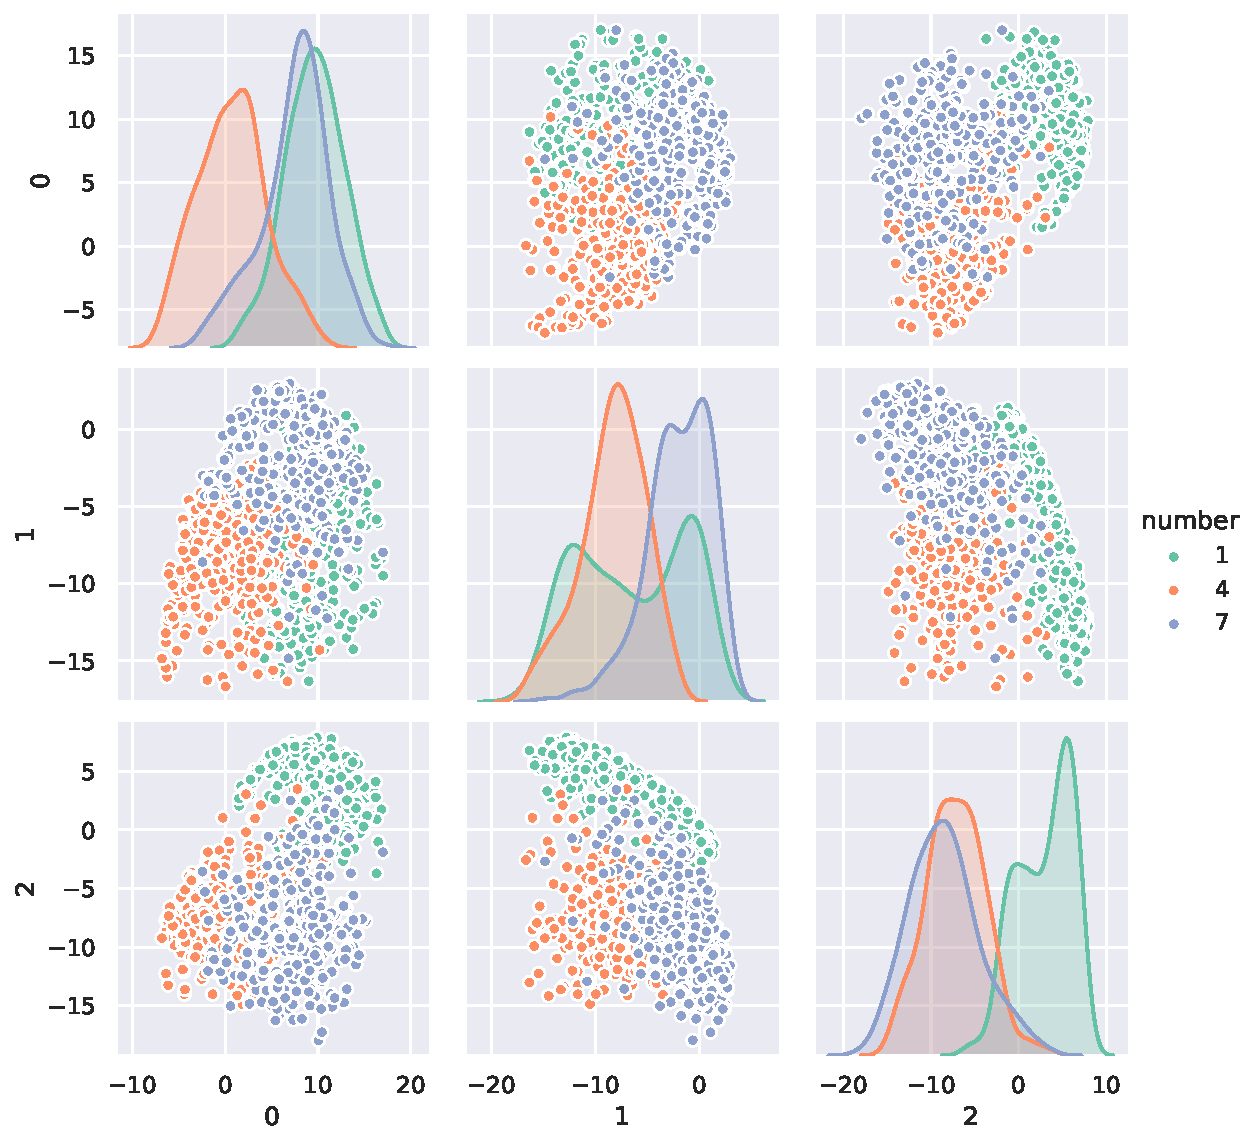
\includegraphics[width=0.3\textwidth]{tex/images/mnist_pca_3D.pdf}}
       \subfloat[]{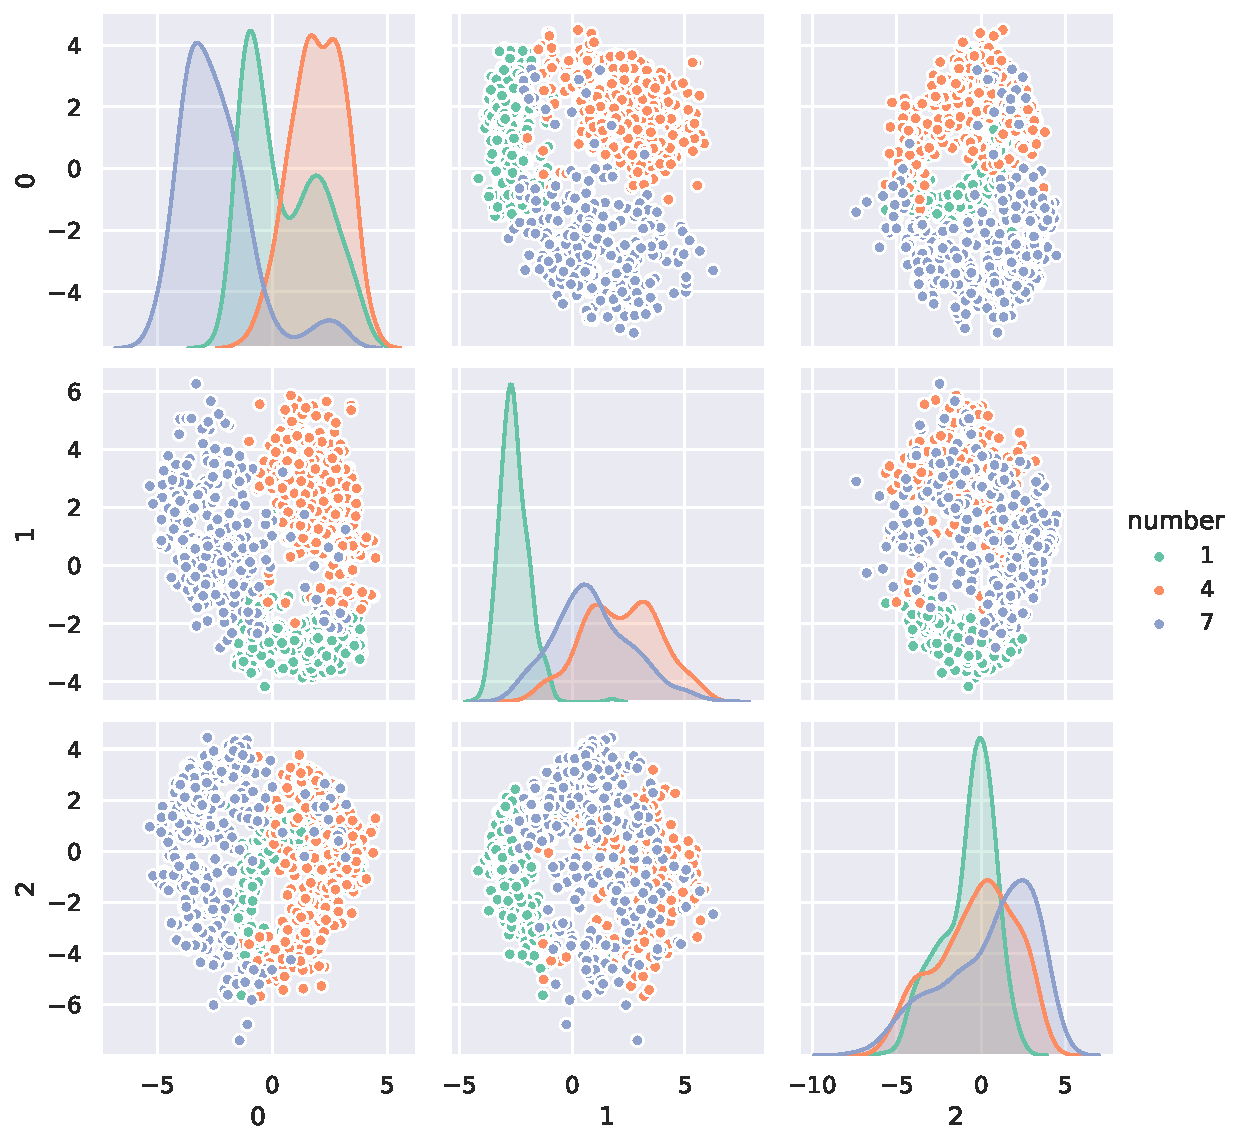
\includegraphics[width=0.3\textwidth]{tex/images/mnist_nlpca_3D.pdf}}
       \subfloat[]{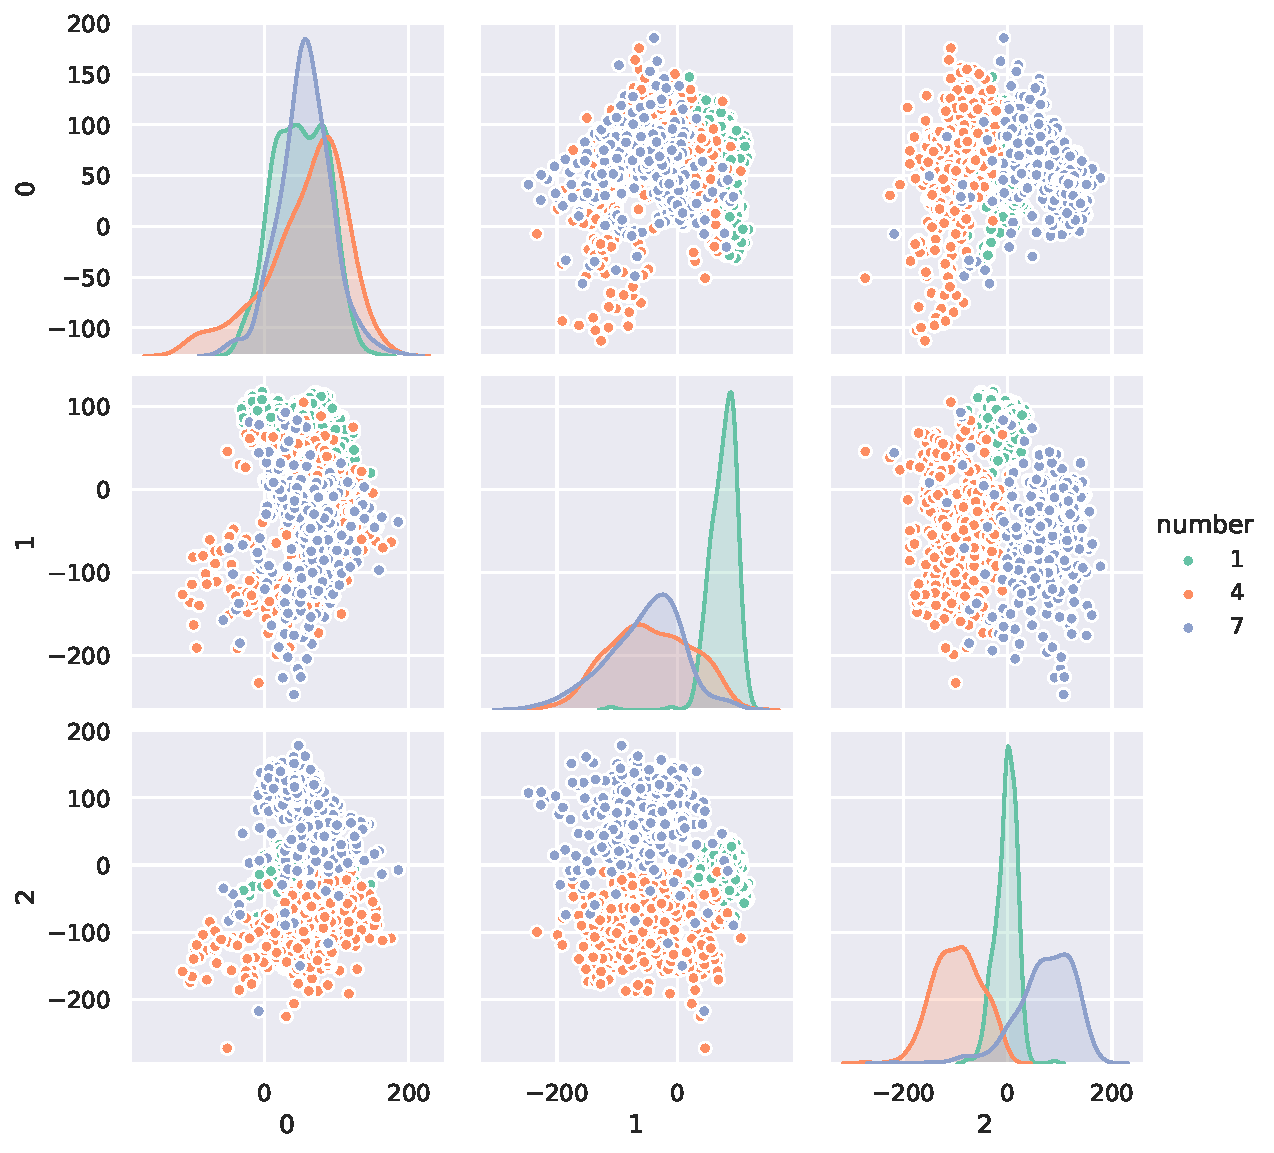
\includegraphics[width=0.3\textwidth]{tex/images/mnist_vae_3D.pdf}}
     \end{figure}
    \end{frame}

    \begin{frame}{BayesPy}
      Flexibilidad en diseño de modelos.

      Altos requisitos de memoria.

      Algoritmo de paso de mensajes variacional.
    \captionsetup[subfigure]{labelformat=empty}
     \begin{figure}[h]
       \centering
         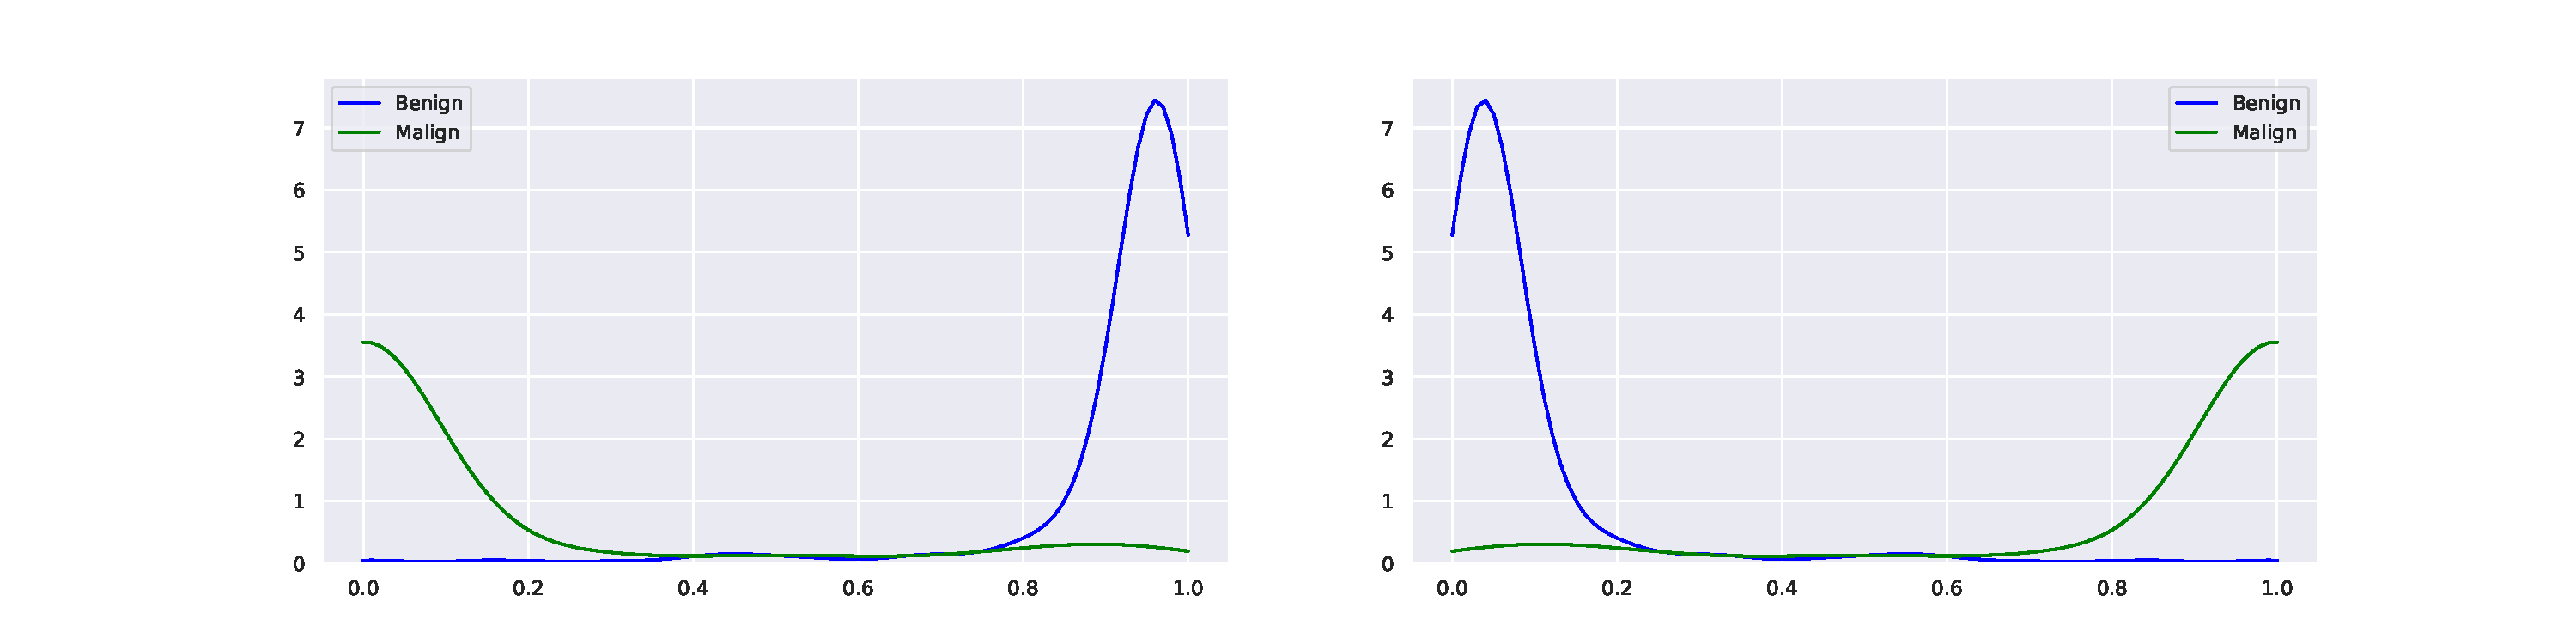
\includegraphics[width=0.9\textwidth]{tex/images/proba_reduced_bayes.pdf}
     \end{figure}
    \end{frame}
    \begin{frame}{Scikit-Learn}

      Modelo de mixtura pre-definido.

      Algoritmo EM.

    \captionsetup[subfigure]{labelformat=empty}
     \begin{figure}[h]
       \centering
         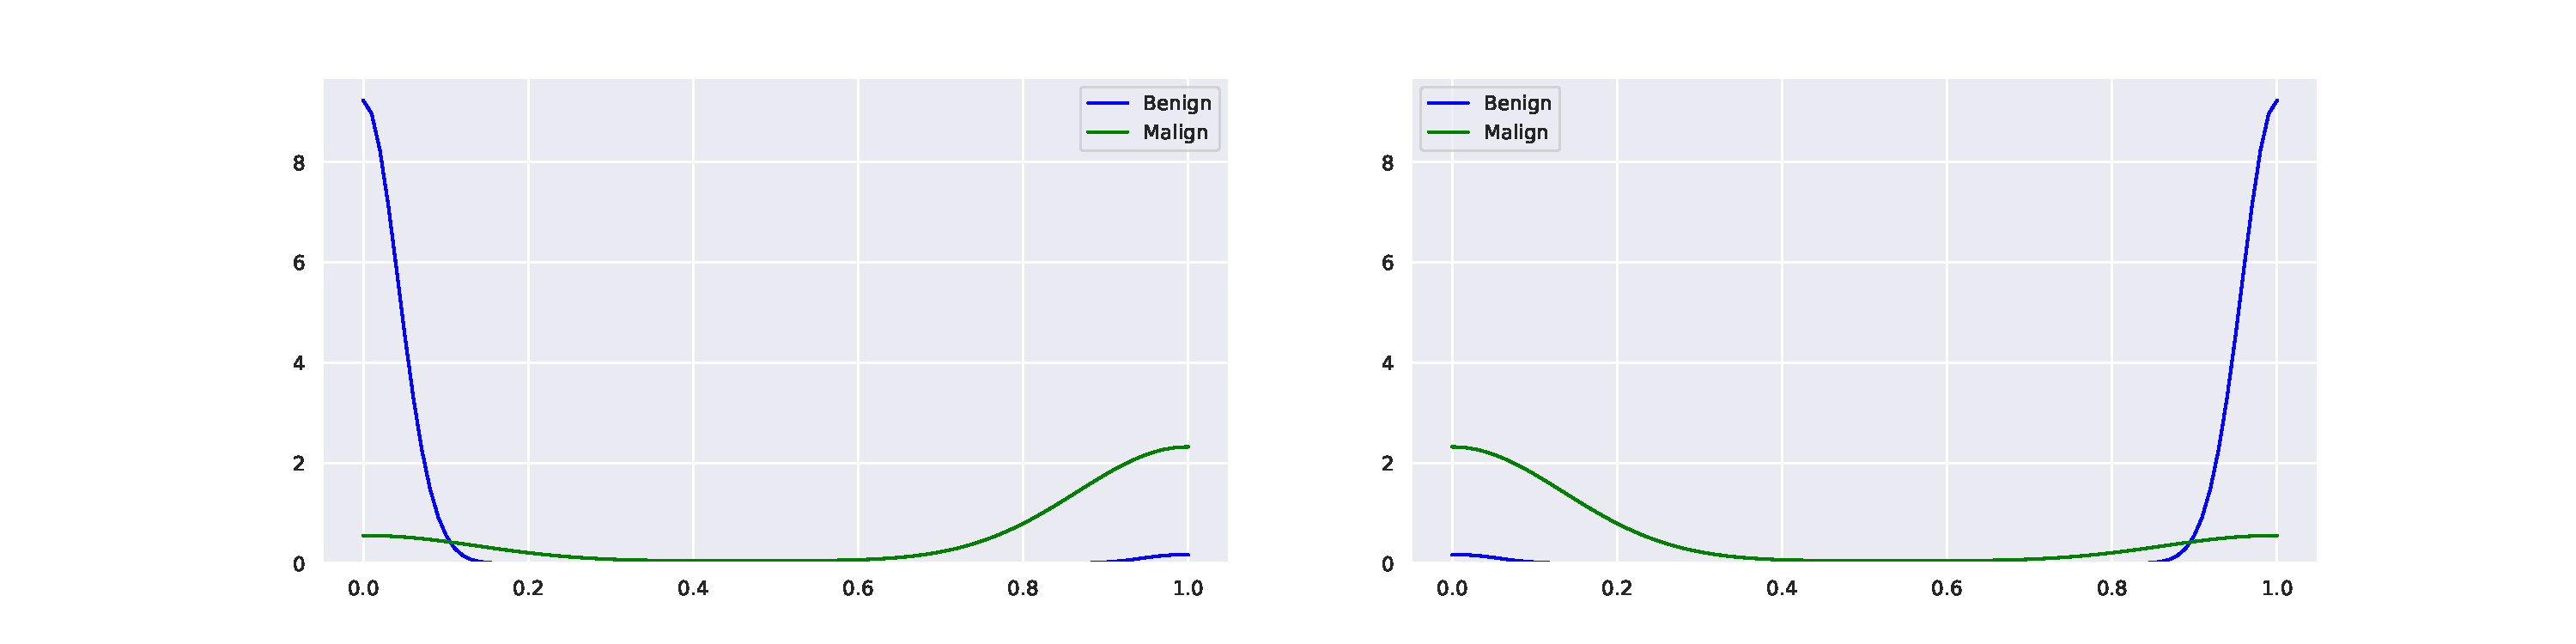
\includegraphics[width=0.9\textwidth]{tex/images/proba_observed.pdf}
     \end{figure}
    \end{frame}


    \begin{frame}{Conclusiones}

      \begin{itemize}
        \item La utilización de modelos gráficos como redes Bayesianas y modelos conjugados en la familia exponencial simplifican la inferencia con variables ocultas hasta su automatización.
        \item Cada software utilizado presenta ventajas e inconvenientes sobre los demás, haciendo que su elección dependa de la tarea que se desee realizar.
      \end{itemize}
    \end{frame}

    \begin{frame}[standout]
      Gracias por su atención
    \end{frame}
\end{document}
